\section{Timeline for project}
For our group this semester project could be split into 6 parts, as seen on \autoref{fig:timeline-for-project}.
There were 4 sprints in total for development of the application. 
For the PO- and process groups there was a lot of work to prepare the first sprint.
This is what we considered \textit{pre sprint 1}.
The process group planned the sprints such that the last sprint would end two weeks before the deadline for handing in the project.
Those last two weeks were spent on usability tests with the customers and finishing the report.
What was common for every sprint was that they followed the process guidelines previously described in \autoref{the-giraf-process}.

\begin{figure}[H]
    \center{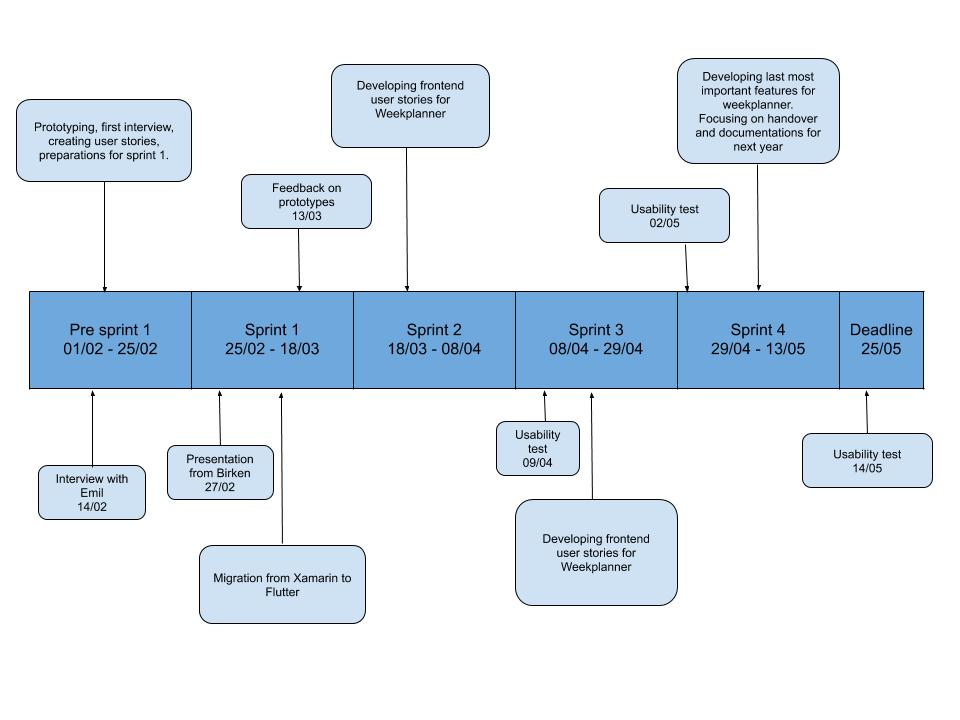
\includegraphics[width=\textwidth]
    {figures/timeline-for-entire-project.JPG}}
    \caption{\label{fig:timeline-for-project} Timeline for the project for our group.}
\end{figure}

\noindent The light blue boxes show the highlights of what was focused on during each sprint by our group.
The different parts will be explained in the following sections.

\subsubsection{Pre sprint 1}
The preparation for the first sprint took place during \textit{pre sprint 1} .
During this time, the groups of the GIRAF project did not fully understand the project, so it was mostly spent gathering information.
We contacted and interviewed customers to gain insight into what the customers wanted.
Based on these interviews, user stories and prototypes were created so that they were ready for sprint 1.
In \textit{pre sprint 1}, an interview with Emil from Egebakken was conducted. 

\subsubsection{Sprint 1}
A presentation from the kindergarten Birken was given on February 27th.
The focus of this sprint started out as fixing bugs and making the application more stable.
It turned out that there were a lot of problems with the frontend with Xamarin, and it was decided that the frontend should be migrated to Flutter during an extraordinary meeting involving most participants of the project.
A meeting was planned with the customers on March 13th to get feedback on the prototypes. 

\subsubsection{Sprint 2}
Sprint 2 was spent developing user stories planned in sprint 1 and some additional user stories for sprint 2.
During this sprint we also implemented some user stories.
At the end of this sprint the first release was completed.
We planned a usability test for this release, but the customers had to cancel this.

\subsubsection{Sprint 3}
At this point the project started to have a some of the most essential features implemented.
In this sprint we focused mostly on implementing user stories and developing new prototypes. 
The sprint ended with the first successful usability test.

\subsubsection{Sprint 4}
As sprint 4 was our final sprint, the sprint mostly focused on completing the user stories that were not completed in the previous sprints and implementing the most essential user stories to have a minimal viable product.
Our group and the process group did not implement any user stories during this sprint, because we focused on documentation and making the handover to next year students as thorough as possible.
In the end of the sprint the final usability test was conducted.

\subsubsection{Deadline}
All development on the weekplanner ended May 13th.
All groups were expected to only focus on finishing their report after this date.
We still needed to finish some documentation for next year, as the last usability tests were held on May 14th and 21st.
Project hand in was on May 28th.
